\documentclass[crop,tikz,border=10px,convert=pdf2svg,multi=false]{standalone}
\usepackage{amsfonts}
\usepackage[defaultsans]{opensans}
\usetikzlibrary{shapes,arrows,positioning}
\begin{document}
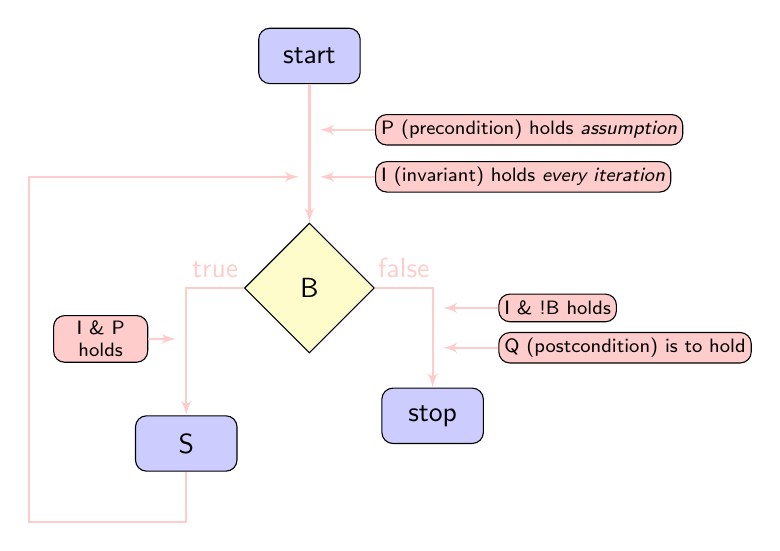
\begin{tikzpicture}[font=\sffamily,node distance=2em,
  decision/.style = {diamond, draw, fill=yellow!20, text width=4em,
    text badly centered, inner sep=0},
  block/.style = {rectangle, draw, fill=blue!20, text centered, text
    width=3em, rounded corners, minimum height=2em},
  cloud/.style = {rectangle, rounded corners, draw, fill=red!20, text centered, minimum
    height=1em, inner sep=0.2em, font=\scriptsize\sffamily},
  line/.style = {draw, -latex', red!20, thick},
  bogus/.style = {draw=none}]

  \node [block] (start) {start};
  \node [decision, below=of start, yshift=-3em] (condition) {B};
  \node [block, below left=of condition, yshift=-2em] (body) {S};
  \node [block, below right=of condition, yshift=-1em] (stop) {stop};

  \draw [line] (start) -- node [bogus,pos=0.33] (a1) {} node
  [bogus,pos=0.67] (a2) {} (condition);

  \draw [line] (condition) -| node[bogus,near start,above] {true} node
  [bogus,pos=0.7] (a3) {} (body);

  \draw [line] (condition) -| node[bogus,near start,above] {false}
  node [bogus,pos=0.6] (a4) {} node [bogus,pos=0.8] (a5) {} (stop);

  \draw [line] (body) |- ++(-2,-1) |- (a2);

  \node [cloud, right=of a1] (a1_txt) {P (precondition) holds \emph{assumption}};
  \node [cloud, right=of a2] (a2_txt) {I (invariant) holds \emph{every iteration}};
  \node [cloud, left=of a3, xshift=1em, text width=3em] (a3_txt) {I \& P holds};
  \node [cloud, right=of a4] (a4_txt) {I \& !B holds};
  \node [cloud, right=of a5] (a5_txt) {Q (postcondition) is to hold};

  \foreach \i in {1,2,...,5} {
    \draw [line] (a\i_txt) -- (a\i);
  }

\end{tikzpicture}
\end{document}
